\subsection{Présentation du Modèle}\label{subsec:presentation-du-modele}
On va se donner des hypothèses simplificatrice à l'échelle economique, la liquidation des banques en defaut est instannée.

On va se fixer une convention d'écriture au cours de cet article.

Soit $n \in \mathbb{N}$,

Considérons $x, y \in \mathbb{R}^n$,

On note :
\begin{align*}
    \min(x,y) &= \min(x_i, y_i) \ \forall i \in \{1,\ldots, n\}\\
    (x)_{+}  &= \max(0, x)
\end{align*}
\textbf{Définition Banque}
\\
Quelques rappels de comptabilité pour faciliter la lecture:
L'actif du bilan représente les possessions de l'entreprise,
son patrimoine, c'est-à-dire ce que la société détient et constitue la
colonne gauche d'un bilan comptable.
Le passif quant à lui est situé à
droite du bilan comptable et représente l'ensemble des dettes de
l'entreprise concernée.
\\
Au cours de cette étude, on nomme banque une entité caractérisée par un bilan simplifié:
Considérons une Banque.

Soit $b \in \mathbb{R}$ et $c \in \mathbb{R}$
\\
On définit $b$ et $c$ respectivement comme la somme totale d'emprunts extérieurs au système bancaire (donc un passif, car dans le
futur on doit rembourser cette dette), et la somme totale de prêts extérieurs au système bancaire (donc un actif).
\\
On définit la somme totale des passifs de la banque:
$$[I]_{i} = \sum_{j=1}^{n} [I]_{ij} + b_i $$
\vspace{0.5cm}
\begin{table}[htbp]
    \centering
    \caption{Bilan comptable simplifié d'une banque dans un réseau interbancaire}
    \label{tab:bilan-banque}
    \begin{tabular}{ |p{2cm}|p{2cm}|  }
        \hline
        \multicolumn{2}{|c|}{Bilan simplifié de la Banque $i$} \\
        \hline
        \textbf{Actifs} & \textbf{Passifs} \\
        \hline
        Prêts interbancaires: $\sum_{j=1}^{n} [I]_{ji}$ & Emprunts interbancaires: $\sum_{j=1}^{n} [I]_{ij}$ \\
        Actifs extérieurs: $c_i$ & Passifs extérieurs: $b_i$ \\
        \hline
        \textbf{Total actifs}: $\sum_{j=1}^{n} [I]_{ji} + c_i$ & \textbf{Total passifs}: $\sum_{j=1}^{n} [I]_{ij} + b_i$ \\
        \hline
        \multicolumn{2}{|c|}{Valeur nette: $\sum_{j=1}^{n} [I]_{ji} + c_i - \sum_{j=1}^{n} [I]_{ij} - b_i$} \\
        \hline
    \end{tabular}
\end{table}
\vspace*{0.5cm}
On nomme ce tableau bilan simplifié car un bilan vérifie la propriété $\text{total d'actif} = \text{total passif}$, ce qui n'est pas forcément notre cas ici.
Puisqu'on a simplement besoin d'observer une banque comme une entité qui reçoit ou donne de l'argent, avec la seule
particularité qu'elle est solvable si et seulement si sa \textbf{Valeur nette} est strictement positive.
\vspace*{0.5cm}
\textbf{Définition: }
On définit un réseau interbancaire comme $\mathcal{R}$, un graphe pondéré orienté avec
$N \in \mathbb{N}$ nœuds, et des flux extérieurs qu'on notera $c$ et $b$, deux vecteurs de $\mathbb{R}^N$.
\\
Soit $I$ la matrice d'exposition bancaire définie par :
$$[I]_{ij} = \begin{cases}
                 \text{obligation} & \text{si $i$ est lié à $j$} \\
                 0 & \text{sinon ou si $i = j$}
\end{cases}$$

Ainsi, un réseau interbancaire est un quadruplet $(\mathcal{R}, I, c, b)$.
\\
Économiquement, on peut interpréter $c$ et $b$ comme les prêts accordés à des entités extérieures au système bancaire (ménages, entreprises) ou des investissements en actifs non-bancaires. La matrice $I$ représente quant à elle l'ensemble des obligations entre banques, formant ainsi le réseau d'interdépendances financières qui peut devenir un canal de contagion en cas de défaut.
\\
Les obligations entre deux banques sont positives ou nulles.
\vspace{0.5cm}
\subsection{Exemple de réseau}\label{subsec:exemple-de-reseau}
Illustrons un exemple d'un réseau interbancaire, avec 4 banques.
On retrouve bien toutes les informations du bilan
simplifié sur la figure~\ref{fig:network_with_externals}.
\begin{figure}[htbp]
    \centering
    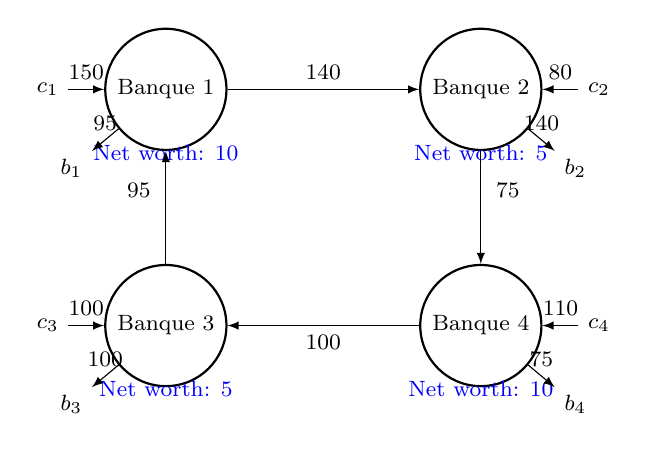
\begin{tikzpicture}[
        bank/.style={circle, draw, thick, minimum size=0.7cm, font=\footnotesize},
        obligation/.style={font=\footnotesize, ->, >=latex},
        external/.style={font=\footnotesize, ->, >=latex},
        networth/.style={font=\footnotesize, text=blue}
    ]
        % Définir les banques (nœuds) - espacement réduit
        \node[bank] (B1) at (0,0) {Banque 1};
        \node[bank] (B2) at (4,0) {Banque 2};
        \node[bank] (B3) at (0,-3) {Banque 3};
        \node[bank] (B4) at (4,-3) {Banque 4};

        % Net worth sous chaque banque
        \node[networth] at (0,-0.8) {Net worth: 10};
        \node[networth] at (4,-0.8) {Net worth: 5};
        \node[networth] at (0,-3.8) {Net worth: 5};
        \node[networth] at (4,-3.8) {Net worth: 10};

        % Définir les obligations interbancaires (lignes droites)
        \draw[obligation] (B1) to node[midway, above] {140} (B2);
        \draw[obligation] (B2) to node[pos=0.35, right=2pt] {75} (B4);  % Ajusté la position
        \draw[obligation] (B4) to node[midway, below] {100} (B3);
        \draw[obligation] (B3) to node[pos=0.65, left=2pt] {95} (B1);  % Ajusté la position

        % Actifs externes (flèches entrantes en pointillé)
        \node[font=\footnotesize] (EA1) at (-1.5,0) {$c_1$};
        \node[font=\footnotesize] (EA2) at (5.5,0) {$c_2$};
        \node[font=\footnotesize] (EA3) at (-1.5,-3) {$c_3$};
        \node[font=\footnotesize] (EA4) at (5.5,-3) {$c_4$};

        \draw[external] (EA1) to node[midway, above] {150} (B1);
        \draw[external] (EA2) to node[midway, above] {80} (B2);
        \draw[external] (EA3) to node[midway, above] {100} (B3);
        \draw[external] (EA4) to node[midway, above] {110} (B4);

        % Passifs externes (flèches sortantes en pointillé)
        \node[font=\footnotesize] (EP1) at (-1.2,-1) {$b_1$};
        \node[font=\footnotesize] (EP2) at (5.2,-1) {$b_2$};
        \node[font=\footnotesize] (EP3) at (-1.2,-4) {$b_3$};
        \node[font=\footnotesize] (EP4) at (5.2,-4) {$b_4$};

        \draw[external] (B1) to node[midway, above] {95} (EP1);
        \draw[external] (B2) to node[midway, above] {140} (EP2);
        \draw[external] (B3) to node[midway, above] {100} (EP3);
        \draw[external] (B4) to node[midway, above] {75} (EP4);
    \end{tikzpicture}
    \caption{Réseau interbancaire avec actifs et passifs externes}
    \label{fig:network_with_externals}
\end{figure}
\textbf{Description}
\begin{itemize}
    \item Banque 1 possède un actif total de 245 (150 d'actifs externes + 95 de prêts interbancaires de la Banque 3) et un passif total de 235 (95 de passifs externes + 140 de prêts à la Banque 2), ce qui explique sa valeur nette positive de 10.
    \item Banque 2 possède un actif total de 220 (80 d'actifs externes + 140 de prêts interbancaires de la Banque 1) et un passif total de 215 (140 de passifs externes + 75 de prêts à la Banque 4), lui donnant une valeur nette de 5.
    \item Banque 3 possède un actif total de 200 (100 d'actifs externes + 100 de prêts interbancaires de la Banque 4) et un passif total de 195 (100 de passifs externes + 95 de prêts à la Banque 1), résultant en une valeur nette de 5.
    \item Banque 4 possède un actif total de 185 (110 d'actifs externes + 75 de prêts interbancaires de la Banque 2) et un passif total de 175 (75 de passifs externes + 100 de prêts à la Banque 3), lui conférant une valeur nette de 10.
\end{itemize}
\textbf{Remarque}
\\
Cette figure~\ref{fig:network_with_externals} est un graphe orienté connexe cyclique.
On peut affirmer avec cette topologie de graphe qu'il est dense, mais ce qui le rend particulièrement intéressant c'est
le cycle, parce que dans cette étude, on souhaite quantifier la résilience d'un réseau en fonction des interconnexions.
Cependant, avant de voir comment construire cela, il faut qu'on garde à l'esprit que le nombre de cycles courts ou longs dans notre réseau influence grandement \textbf{l'effet de cascade}
de défaut; d'ailleurs ce sera une difficulté au cours de cette étude, de faire la part des choses entre le rôle de la densité du réseau et le nombre de cycles présents dans le réseau.
\subsection{Approche par Simulation}\label{subsec:approche-par-simulation}
Avec les notations définies précédemment,
on met en place un réseau afin de le tester, c'est-à-dire appliquer un choc exogène sur le réseau.
\textbf{On définit un choc comme le non-remboursement d'une entité extérieure vers une banque}, c'est-à-dire lorsque le $c_i$ (actif extérieur de la banque i) attendu diminue.

\textbf{Choix du Graphe}

\textbf{Graphe de Erdos-Renyi dirigé}
Dans la théorie des graphes aléatoires, on va considérer un graphe orienté $\mathcal{R}$ avec $n \in \mathbb{N}$ comme nombre de nœuds.
Notons :
$$\mathcal{N} = \{1,\ldots, n\} $$
l'ensemble des nœuds de $\mathcal{R}$.

Notons $p \in [0,1]$ la probabilité qu'il y ait une arête entre deux nœuds de $\mathcal{N}$, identique pour tous les nœuds.
On suppose de plus qu'il y a indépendance pour le lien entre chaque nœud.

Ce type de graphe aléatoire est un célèbre graphe nommé Graphe d'Erdos-Renyi (qui n'est pas forcément orienté dans sa définition générale).

On choisit de faire un choc exogène car cela nous permet de formaliser une mesure simple de gravité du choc.
Soit $x\in \mathbb{R}^N$ un choc, notons que :
$$\forall i \in \{1, \ldots, N\} \ x_i \in [0, c_i]$$
Ainsi on définit la gravité du choc x, notée g telle que :
$$g = \frac{\|x\|}{\|c\|}$$
avec $\|x\| = \sum_{i=1}^{n} |x_i|$\\
De plus $g \in [0, 1]$.

En considérant cette mesure de gravité du choc, on souhaite voir la relation avec la proportion de défaut notée $d$
pour un $p$ fixé, la probabilité dans le graphe d'Erdos-Renyi d'avoir un lien entre deux banques.
On défini $d$ tel que :
$$d = \frac{\text{Nombre de defaut}}{N}$$
On voit naturellement que d'un point de vue empirique, la simulation s'exprime d'elle-même : on va tester, pour un choc exogène croissant linéaire avec un réseau de plus en plus dense (faire croître p), la courbe
de la proportion de défaut dans le réseau après avoir appliqué le choc.
\\\\
Pour faire cela, on a choisi de faire une implémentation en Python avec une architecture MVC (modèle, vue et contrôleur), pour un développement modulaire qui nous aidera dans de futurs développements du modèle du réseau, sans trop
notons en l'occurence que ce choix est très adapté pour ce type de problème, car une simulation par définition est un objet qui prend différent objet et teste des propriété dessus.
Notre simulateur étant le controlleur, il va prendre un réseau qui est une donnée avec toute sa logique metier, et va appliquer des chocs sur le reseau, ensuite demande à la vue de nous afficher le graphique correspondant.\\
À ce niveau, on peut déjà se demander si cette approche nous donnera une bonne mesure du risque systémique.
À quoi ressemblerait cette mesure ?
\\
\textbf{Avec un réseau, avec ses paramètres et sa topologie, en l'occurrence pour nous avec la densité du réseau, faire ressortir la résilience du réseau, qui est un seuil de proportion de défaut, qui lorsqu'on le dépasse, on considère qu'on est en crise systémique.}
En l'état actuel de l'étude, on n'a pas encore traduit cela en probabilité, c'est-à-dire la probabilité pour un réseau de faire une crise systémique, car pour cela on devrait considérer la probabilité d'avoir un choc particulier.
\\\\
Il nous manque un ingredient pour que cette simulation se déroule bien, comment mettre à jour le réseau et compter le nombre de defaut après un choc ?\\
Revenons sur la figure~\ref{fig:network_with_externals}, si la banque 1 fait défaut car on ne lui rembourse plus 150 mais 5, un calcul rapide de sa valeur nette nous montre qu'il
est en defaut.
Avec cette perte énorme de capital pour la banque 1, on a un autre problème qui apparait, maintenant que banque 1 à fait défaut, elle ne peut plus rembourser ces dettes en totalité.
Une méthode utilisé en finance dans ce cas, c'est la liquidation par prorata, rembourser nos créanciers en fonction de la proportion de leurs créances dans nos dettes.

\subsection{Algorithme du vecteur de payement}
Ainsi donc on défini une matrice R, qui va representer la proportion de chaque dette:
$$[R]_{ij} = \frac{[I]_{ij}}{[I]_{i}}$$
Reprenons l'exemple~\ref{subsec:exemple-de-reseau}, si Banque 1 ne rembourse que 60 (on arrondi) à la Banque 2, ce qui mène la Banque 2 à également faire défaut, par le même proceder,
elle ne remboursera que 49 à la banque 4, ce qui la mène aussi à faire defaut, et de même,
la banque 4 rembourse 75 à la banque 3, qui elle aussi se retrouvera en defaut.
Mais tous ce calcul n'a été effectuer en supposant que la banque 3 rembourse la totalité de sa dette à la banque 1, ainsi on voit ici un problème de payements.
Le vecteur de payement qui nous permet d'avoir le vecteur de payement d'équilibre est un point fixe d'une transformation défini dans le papier~\cite{eisenberg2001systemic} et reformuler par noe dans \cite{peyton2016contagion},
On rappel cette transformation notée $\phi(P)$, avec P un vecteur de payement.
Notons $\bar{P} \in \mathbb{R}^N$ défini tel que:
$$\bar{P}_i = [I]_i$$
Avant de donner la formule, on peut l'intuité economiquement, pour une banque i, elle ne va pas rembourser plus qu'elle devait de base, de plus elle ne peut pas rembourser une somme qu'elle ne possède pas.
Ainsi on en déduit la formule :
$$\phi(P) = \min(\bar{P}, \max(0, R^{T}P + c))$$
Ainsi le vecteur de payement d'équilibre est une solution du problème de point de fixe $\phi(P) = P$.

C'est là que l'algorithme d'Eisenberg-Noe intervient, car dans leur papier \cite{eisenberg2001systemic}, il démontre que dans les conditions qu'on vérifie par construction, on commence avec un reseau qui contient des banques avec des valeurs nette
positives et les poids sur les noeuds sont positifs, ce que l'algorithme de noe demande pour la convergence du probleme.

Maintenant avec cette algorithme, on va voir ce que les tracer nous donne.

